\documentclass[compress,red]{beamer}
\mode<presentation>
\setbeamertemplate{navigation symbols}{}
\usetheme{Warsaw}
%\setbeameroption{show notes}
%\setbeameroption{show only notes}
\setbeameroption{hide notes}

%\hypersetup{pdfpagemode=FullScreen} % makes your presentation go automatically to full screen
\useoutertheme[subsection=false]{smoothbars}

% include packages
\usepackage{subfigure}
\usepackage{multicol}
\usepackage{amsmath}
\usepackage{epsfig}
\usepackage{graphicx}
\usepackage[all,knot]{xy}
\xyoption{arc}
\usepackage{url}
\usepackage{multimedia}
\usepackage{hyperref}
\usepackage{helvet}
\usepackage[polish,english]{babel}
\usepackage[utf8]{inputenc}
\usepackage{multirow}
\usepackage{verbatim}
%\usepackage{geometry}
%\geometry{verbose,letterpaper}
%\usepackage{movie15}
%\usepackage{hyperref}
\usepackage{pgfpages}


\titlegraphic{\scalebox{4}{
    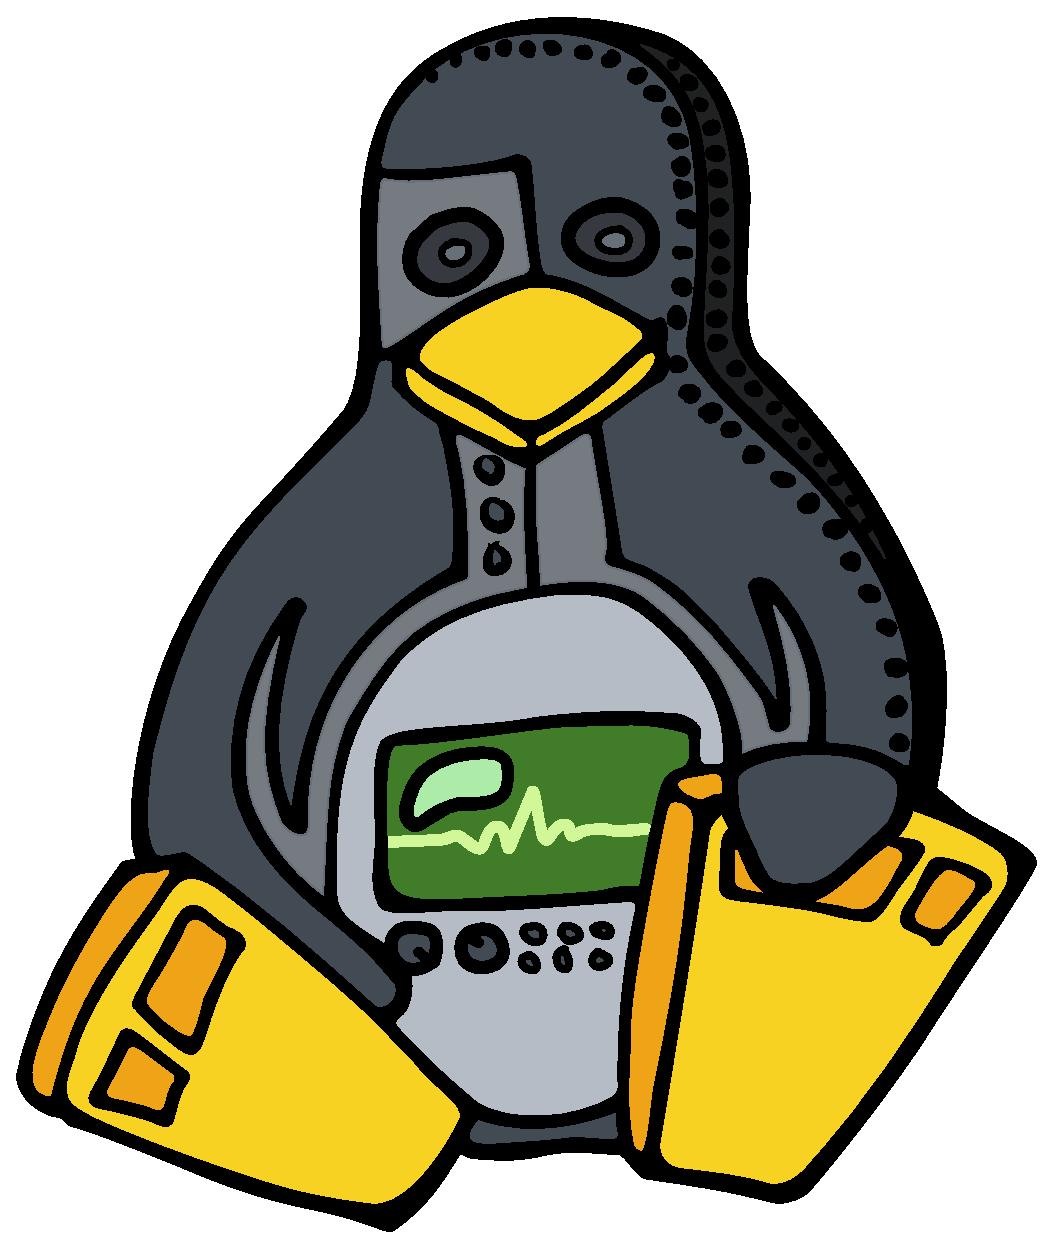
\includegraphics[height=0.5cm]{../pictures/ohr_logo.eps}~
    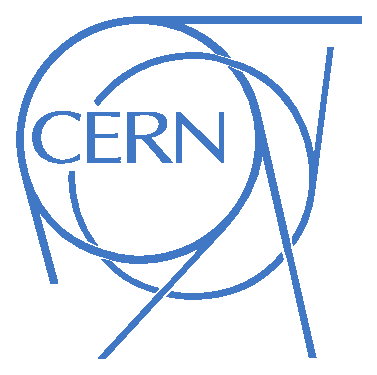
\includegraphics[height=0.5cm]{../pictures/cern_logo.eps}}
}


\title[CERN's FMC kit] % (optional, use only with long paper titles)
{CERN's FMC kit}


\author[Matthieu Cattin] % (optional, use only with lots of authors)
{\mbox{Matthieu Cattin}, \mbox{Evangelia Gousiou}, \mbox{Javier Serrano}, \mbox{Erik van der Bij}, \mbox{Tomasz W\l{}ostowski}}

\institute
{
%  BE-CO Hardware and Timing section\\
  CERN, Geneva, Switzerland
 }

\date[ICALEPCS 2013] %(optional, should be abbreviation of conference name)
{ICALEPCS 2013, San Francisco, 9 October 2013}


%\subject{Theoretical Computer Science}
% This is only inserted into the PDF information catalog. Can be left
% out.

% If you have a file called "university-logo-filename.xxx", where xxx
% is a graphic format that can be processed by latex or pdflatex,
% resp., then you can add a logo as follows:

%\pgfdeclareimage[height=1cm]{ohr-logo}{ohr_logo.jpg}
%\logo{\pgfuseimage{ohr-logo}}


% Delete this, if you do not want the table of contents to pop up at
% the beginning of each subsection:
\AtBeginSection[]
{
  \begin{frame}<beamer>{Outline}
    \tableofcontents[currentsection]
  \end{frame}
}


% If you wish to uncover everything in a step-wise fashion, uncomment
% the following command:
%\beamerdefaultoverlayspecification{<+->}



\begin{document}

%------------ FRAME --------------------------------------------------
\begin{frame}

  \titlepage

  \note[item]{Good morning everyone.}
  \note[item]{I work at CERN in the Beam Controls group.}
  \note[item]{We provide electronics to other groups.}
  \note[item]{Four year ago we changed the way we develop hardware.}
  \note[item]{I will present the FMC kit we develop using new methods.}

\end{frame}

%------------ FRAME --------------------------------------------------
\begin{frame}{Outline}

  \tableofcontents
  % You might wish to add the option [pausesections]

  \note[item]{First I will a new kit.}
  \note[item]{Then I will introduce Open Hardware and HOW we use it.}
  \note[item]{Then I will present our Open Hardware products.}
  \note[item]{I will also present the architecture of the gateware inside the FPGA and the new tools and concepts we developed.}
  \note[item]{And I will finish with some conclusions.}

\end{frame}


% Structuring a talk is a difficult task and the following structure
% may not be suitable. Here are some rules that apply for this
% solution:

% - Exactly two or three sections (other than the summary).
% - At *most* three subsections per section.
% - Talk about 30s to 2min per frame. So there should be between about
%   15 and 30 frames, all told.

% - A conference audience is likely to know very little of what you
%   are going to talk about. So *simplify*!
% - In a 20min talk, getting the main ideas across is hard
%   enough. Leave out details, even if it means being less precise than
%   you think necessary.
% - If you omit details that are vital to the proof/implementation,
%   just say so once. Everybody will be happy with that.



%#####################################################################
%############ SECTION ################################################
\section{Why a new kit}

\subsection*{} % dummy subsection to display dots

%------------ FRAME --------------------------------------------------
\begin{frame}{CERN Beams Controls group}

  \begin{block}{Responsible for}
    \begin{itemize}
    \item Specification, design, procurement and operation of electronic modules
    \item Linux device drivers, C/C++ libraries, test programs
    \end{itemize}
  \end{block}

  \begin{block}{Hardware kit}
    \begin{itemize}
    \item Analog and digital I/O
    \item Level converters, repeaters
    \item Serial links, timing modules
    \end{itemize}
  \end{block}

  \begin{block}{Currently, October 2013}
    \begin{itemize}
    \item About 120 module types % -- with just a few engineers
    \item Most are custom designed: only 1 in 4 is commercial
    \end{itemize}
  \end{block}

  \note[item]{So, why a new kit?}
  \note[item]{Let me first introduce the Hardware and Timing section.}
  \note[item]{The hardware and timing section of the beams controls group is responsible for the whole chain of electronics modules design; from specification to operation in the accelerators.}
  \note[item]{The section is also responsible to provide Linux drivers, with libraries and test programs for the hardware boards.}
  \note[item]{The hardware kit or the set of modules we have to maintain contains modules like: analog and digital I/O, level converters, timing modules, etc...}
  \note[item]{And currently we have more than 100 different modules and most of them are custom designs.}

\end{frame}

\begin{comment}
%------------ FRAME --------------------------------------------------
\begin{frame}{Why a new kit?}

  \begin{block}{Motivations to design a new kit}
    \begin{itemize}
    \item Current kit hard to maintain.
    \item Obsolete components/modules.
    \item Limited stock $\rightarrow$ no new installations.
    \item Incomplete/nonexistent documentation.
    \item Large variety of modules (about 120).
    \item No re-use strategy (pcb, hdl).
    \item \textit{Ad hoc}/non-standard interfaces. %(buses, serial protocols, etc...)
    \end{itemize}
  \end{block}

  \note[item]{So with such a big kit, why do we design a new one?}
  \note[item]{The main reasons are because the current kit is hard to maintain.}
  \note[item]{It contains a lot of obsolete components or modules.}
  \note[item]{Most of the time the documentation is incomplete or lost.}
  \note[item]{Our engineer team is very small to support this large variety of modules.}
  \note[item]{And finally, we didn't have any re-use strategy and most of the interfaces of old modules are non-standard.}

\end{frame}
\end{comment}

%------------ FRAME --------------------------------------------------
\begin{frame}{Why a new kit?}

  \begin{block}{Motivations to design a new kit}
    \begin{itemize}
    \item Obsolete components/modules
    \item Limited stock $\rightarrow$ no new installations
    \item Incomplete/nonexistent documentation
    \end{itemize}
  \end{block}

  \begin{block}{New approach}
    \begin{itemize}
    \item Open and modular designs
    \item Compliant with existing standards
    \end{itemize}
  \end{block}

  \begin{block}{Carrier-mezzanine concept}
    \begin{itemize}
%    \item Generic platform-dependent carriers
%    \item Specific platform-independent mezzanines
    \item Reduce number of supported modules
    \item Only one complex design per platform (carrier)
    \end{itemize}
  \end{block}

  \note[item]{So to make the new kit better, we followed some principles like: keeping designs open and modular and based on standards.}
  \note[item]{As we have to support several platforms, we decided to go for a carrier-mezzanine concept.}
  \note[item]{this will allow us to reduce the number of module.}
  \note[item]{And also to design a complex carrier board only once for each platform.}

\end{frame}

%------------ FRAME --------------------------------------------------
\begin{frame}{Use of standards}

  \begin{block}{Based on standards}
    \begin{itemize}
    \item Platform bus: VME, PCI, PCIe, PXIe
    \item FMC (FPGA Mezzanine Card, ANSI/VITA 57.1)
    \item Wishbone FPGA internal bus
    \item Linux device drivers
    \end{itemize}
  \end{block}

  \begin{block}{Contribute to standards}
    \begin{itemize}
    \item Wishbone pipelined mode: Wishbone spec Rev.B4 (2010)
    \item FMC bus Linux driver structure: in Linux v3.11
    \item ZIO Linux framework for DAQ and CTL hardware: \\ RFC made to Linux Kernel list
    \end{itemize}
  \end{block}

  \note[item]{As I said, our new kit is based on standards.}
  \note[item]{For the platform bus we use: VME, PCI, PCIe, and PXIe.}
  \note[item]{For the carrier mezzanine concept, we use the FMC standard.}
  \note[item]{For the FPGA internal bus we use Wishbone.}
  \note[item]{And for the drivers we use Linux.}
  \note[item]{We also contributed to standards.}
  \note[item]{For example a pipeline mode for Wishbone and new features in the Linux kernel.}

\end{frame}


%#####################################################################
%############ SECTION ################################################
\section[Introduction to OH]{Introduction to Open Hardware}

\subsection*{} % dummy subsection to display dots

%------------ FRAME --------------------------------------------------
\begin{frame}{Why we use Open Hardware}

  \begin{block}{Fully specify the design}
    \begin{itemize}
    \item Avoid black boxes.
    \end{itemize}
  \end{block}

  \begin{block}{Better designs}
    \begin{itemize}
    \item Peer review by experts, including companies.
    \end{itemize}
  \end{block}

  \begin{block}{Knowledge sharing by design re-use}
    \begin{itemize}
    \item One of CERN's key mission.
    \item Stimulates collaborations, inside and outside CERN.
    \end{itemize}
  \end{block}

  \begin{block}{Healthier relationship with companies}
    \begin{itemize}
    \item No vendor-locked situations.
    \item Small companies can play important role.
    \end{itemize}
  \end{block}

  \note[item]{Why did we decided to go for open hardware?}
  \note[item]{Because we don't want to support black boxes in operation.}
  \note[item]{Because our design will become better with peer review.}
  \note[item]{Because one of the cern's key mission is knowledge sharing and an open design have more chance to be re-used.}
  \note[item]{And finally to have healthier relation with companies.}

\end{frame}

%------------ FRAME --------------------------------------------------
\begin{frame}{OH repository and license}

  \begin{block}{Open Hardware Repository \href{http://ohwr.org}{-- ohwr.org}}
    \begin{itemize}
    \item Web-based collaborative tool for electronics designers
    \item Wiki, News, File repository, Issues management, Mailing list
    \item Readable by everyone, without registration
   \end{itemize}
  \end{block}

  \begin{block}{CERN Open Hardware License \href{http://ohwr.org/cernohl}{-- ohwr.org/cernohl}}
    \begin{itemize}
    \item Developed by Knowledge Transfer Group at CERN.
    \item Better suited than non-HW licenses (GPL, Creative Commons\dots)
    \item Defines conditions for using and modifying licensed material.
   \end{itemize}
  \end{block}

  \note[item]{In order to help collaboration, we created the open hardware repository.}
  \note[item]{It's a website where the designs are stored and are accessible by everyone.}
  \note[item]{As we couldn't find any suitable license for our design, we created a new one called CERN OHL}

\end{frame}



%#####################################################################
%############ SECTION ################################################
\section[OH products]{Open Hardware products}
%?? CERN Open Hardware products

\subsection*{} % dummy subsection to display dots

%------------ FRAME --------------------------------------------------
\begin{frame}{Open Hardware products}

  \begin{block}{More than just a board}
    \begin{itemize}
    \item Hardware board
    \item FPGA gateware
    \item Linux driver
    \item Production test system
    \end{itemize}
  \end{block}

  \begin{block}{Carriers}
    \begin{itemize}
    \item Three fully supported (VME, PCIe, PXIe)
    \item Six other carriers (VXS, AMC, stand-alone)
    \end{itemize}
  \end{block}

  % VFC, PFC, AFC, RHINO, VXS DSP carrier, Stand-alone 18-slot FMC carrier

  \begin{block}{Mezzanines}
    \begin{itemize}
    \item Four fully supported (ADC-100M, TDC, DIO-5ch, FD)
    \item About a dozen other mezzanines (ADC, DAC, DDS, DIO)
    \end{itemize}
  \end{block}

  % ADC-130M, ADC-200k, ADC-250M, ADC-1G
  % ADC-125M-DAC-600M, ADC-10M-DAC-50M
  % DAC-10M, DAC-130M, DAC-250M, DAC-600M-DDS
  % DIO-16ch, DIO-32ch
  % + others more specific mezzanines

  \note[item]{The new hardware kit is not only about hardware boards.}
  \note[item]{You can see it like a set of products.}
  \note[item]{With FPGA gateware, Linux driver and test system.}
  \note[item]{So far we fully support 2 carrier, one VME and one PCIe.}
  \note[item]{And 4 mezzanines, an ADC 100MSPS, a TDC, a Digital IO and a fine delay.}
  \note[item]{But there are many more designs available on the open hardware repository website.}

\end{frame}

%------------ FRAME --------------------------------------------------
\begin{frame}{SVEC - Simple VME FMC Carrier}{Commercialised in Germany}

  \begin{center}
    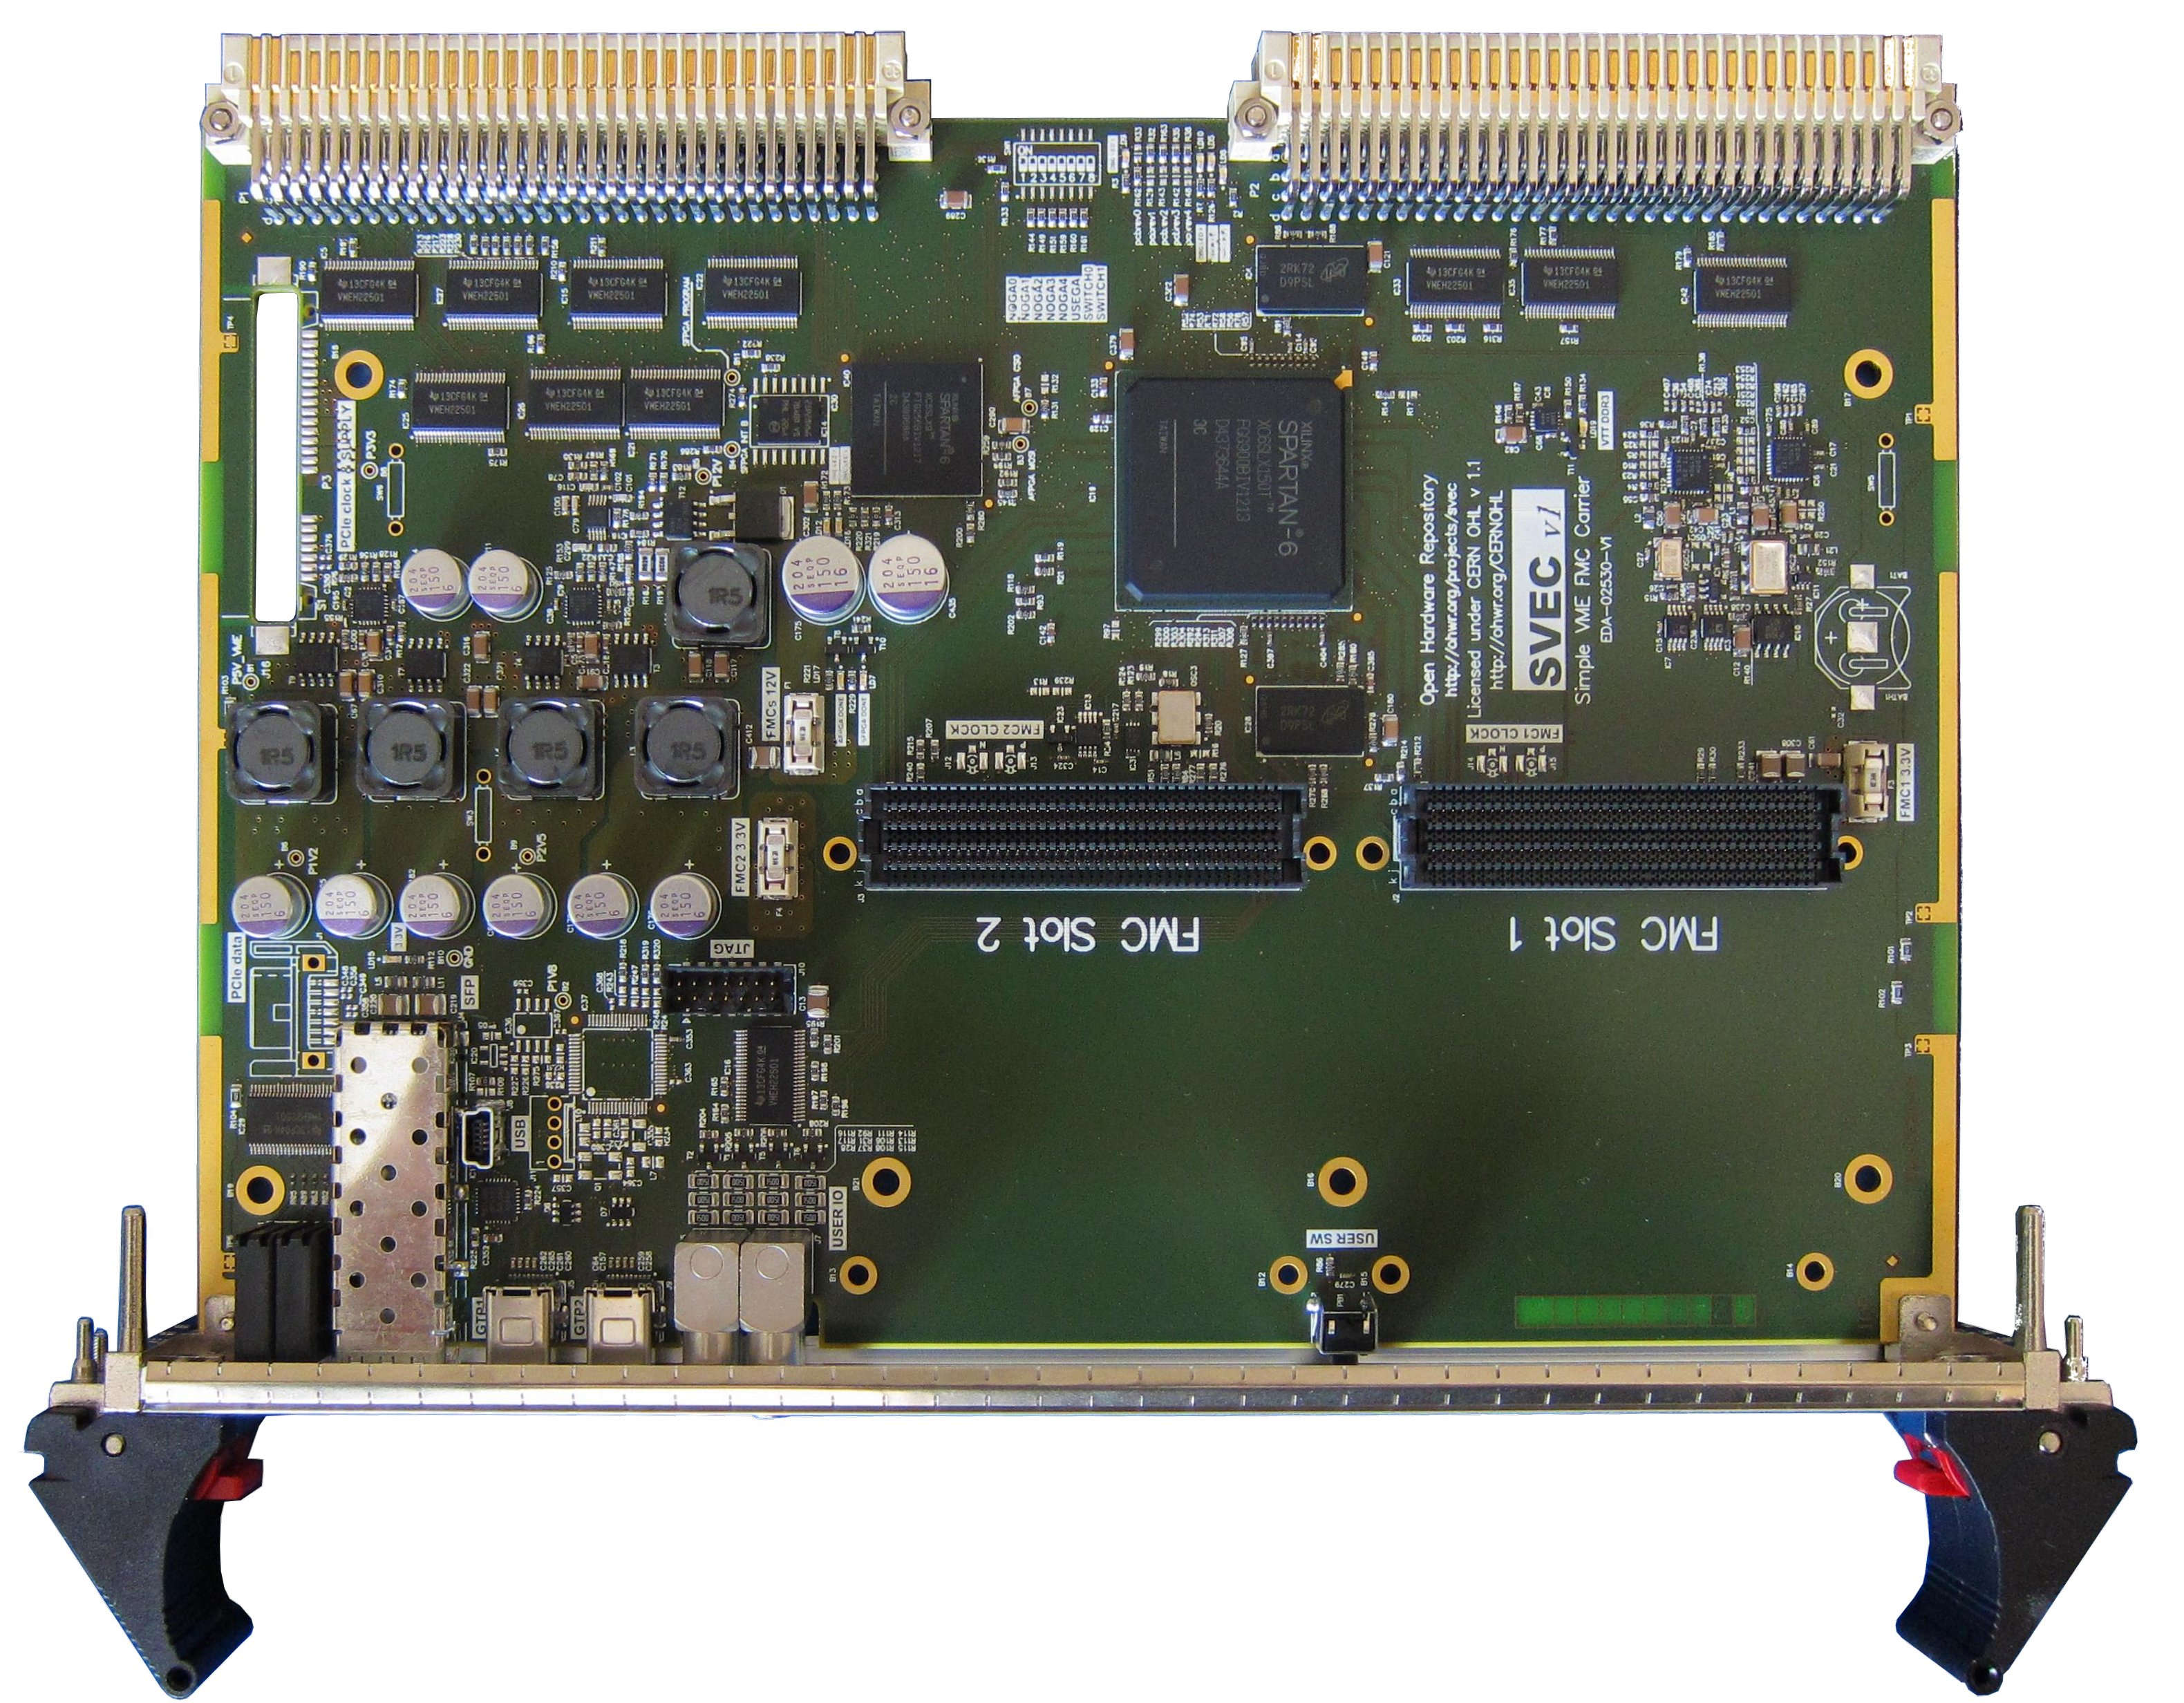
\includegraphics[height=7cm]{../pictures/svec.eps}
  \end{center}

  \note[item]{This is our VME carrier, with 2 FMC slots.}

\end{frame}

%------------ FRAME --------------------------------------------------
\begin{frame}{SPEC - Simple PCI Express FMC carrier}{Commercialised in Spain, The Netherlands \& Poland}

  \begin{center}
    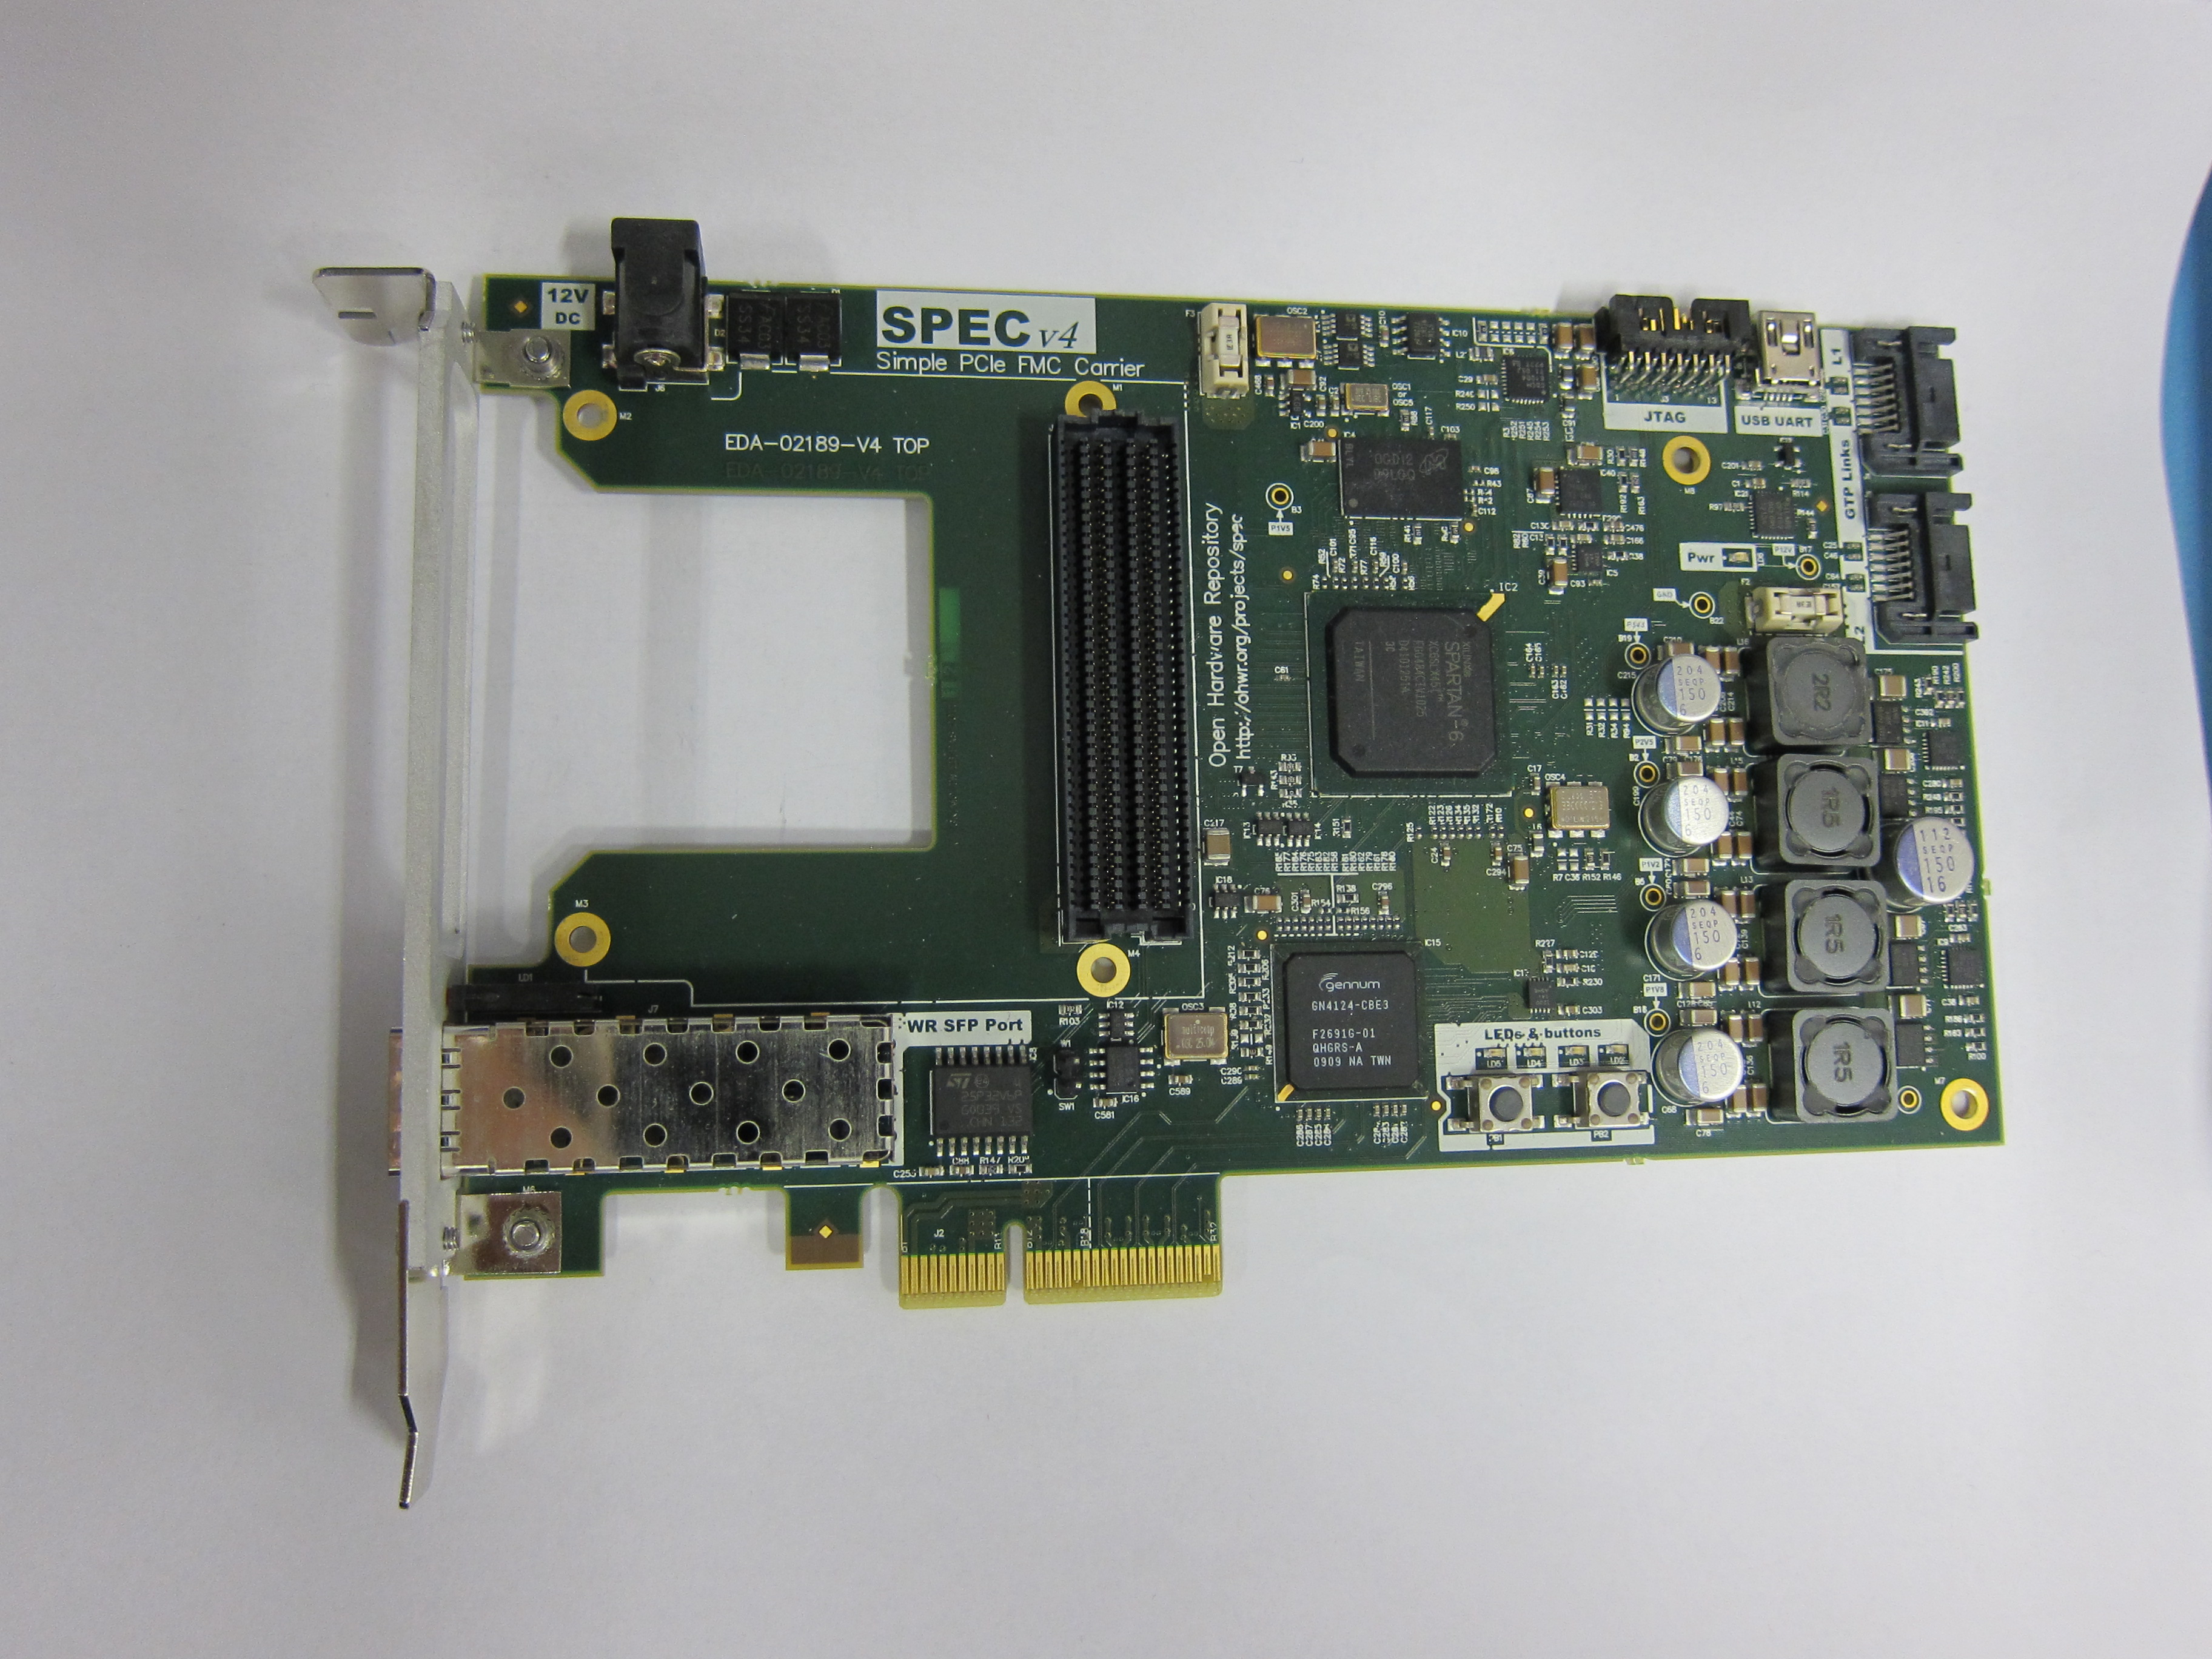
\includegraphics[height=7cm]{../pictures/spec_v4.eps}
  \end{center}

  \note[item]{This is our PCIe carrier, with only 1 FMC slot.}

\end{frame}

%------------ FRAME --------------------------------------------------
\begin{frame}{SPEXI - Simple PXI Express FMC carrier}{A modified SPEC board}

  \begin{center}
    \includegraphics[height=7cm]{../pictures/spexi_v0.eps}
  \end{center}

  \note[item]{This a PXIe carrier based on the PCIe.}

\end{frame}

%------------ FRAME --------------------------------------------------
\begin{frame}{FMC mezzanine: 5-channel 1ns TDC}{A joint development by TE/ABT, TE/CRG \& BE/CO}

  \begin{center}
    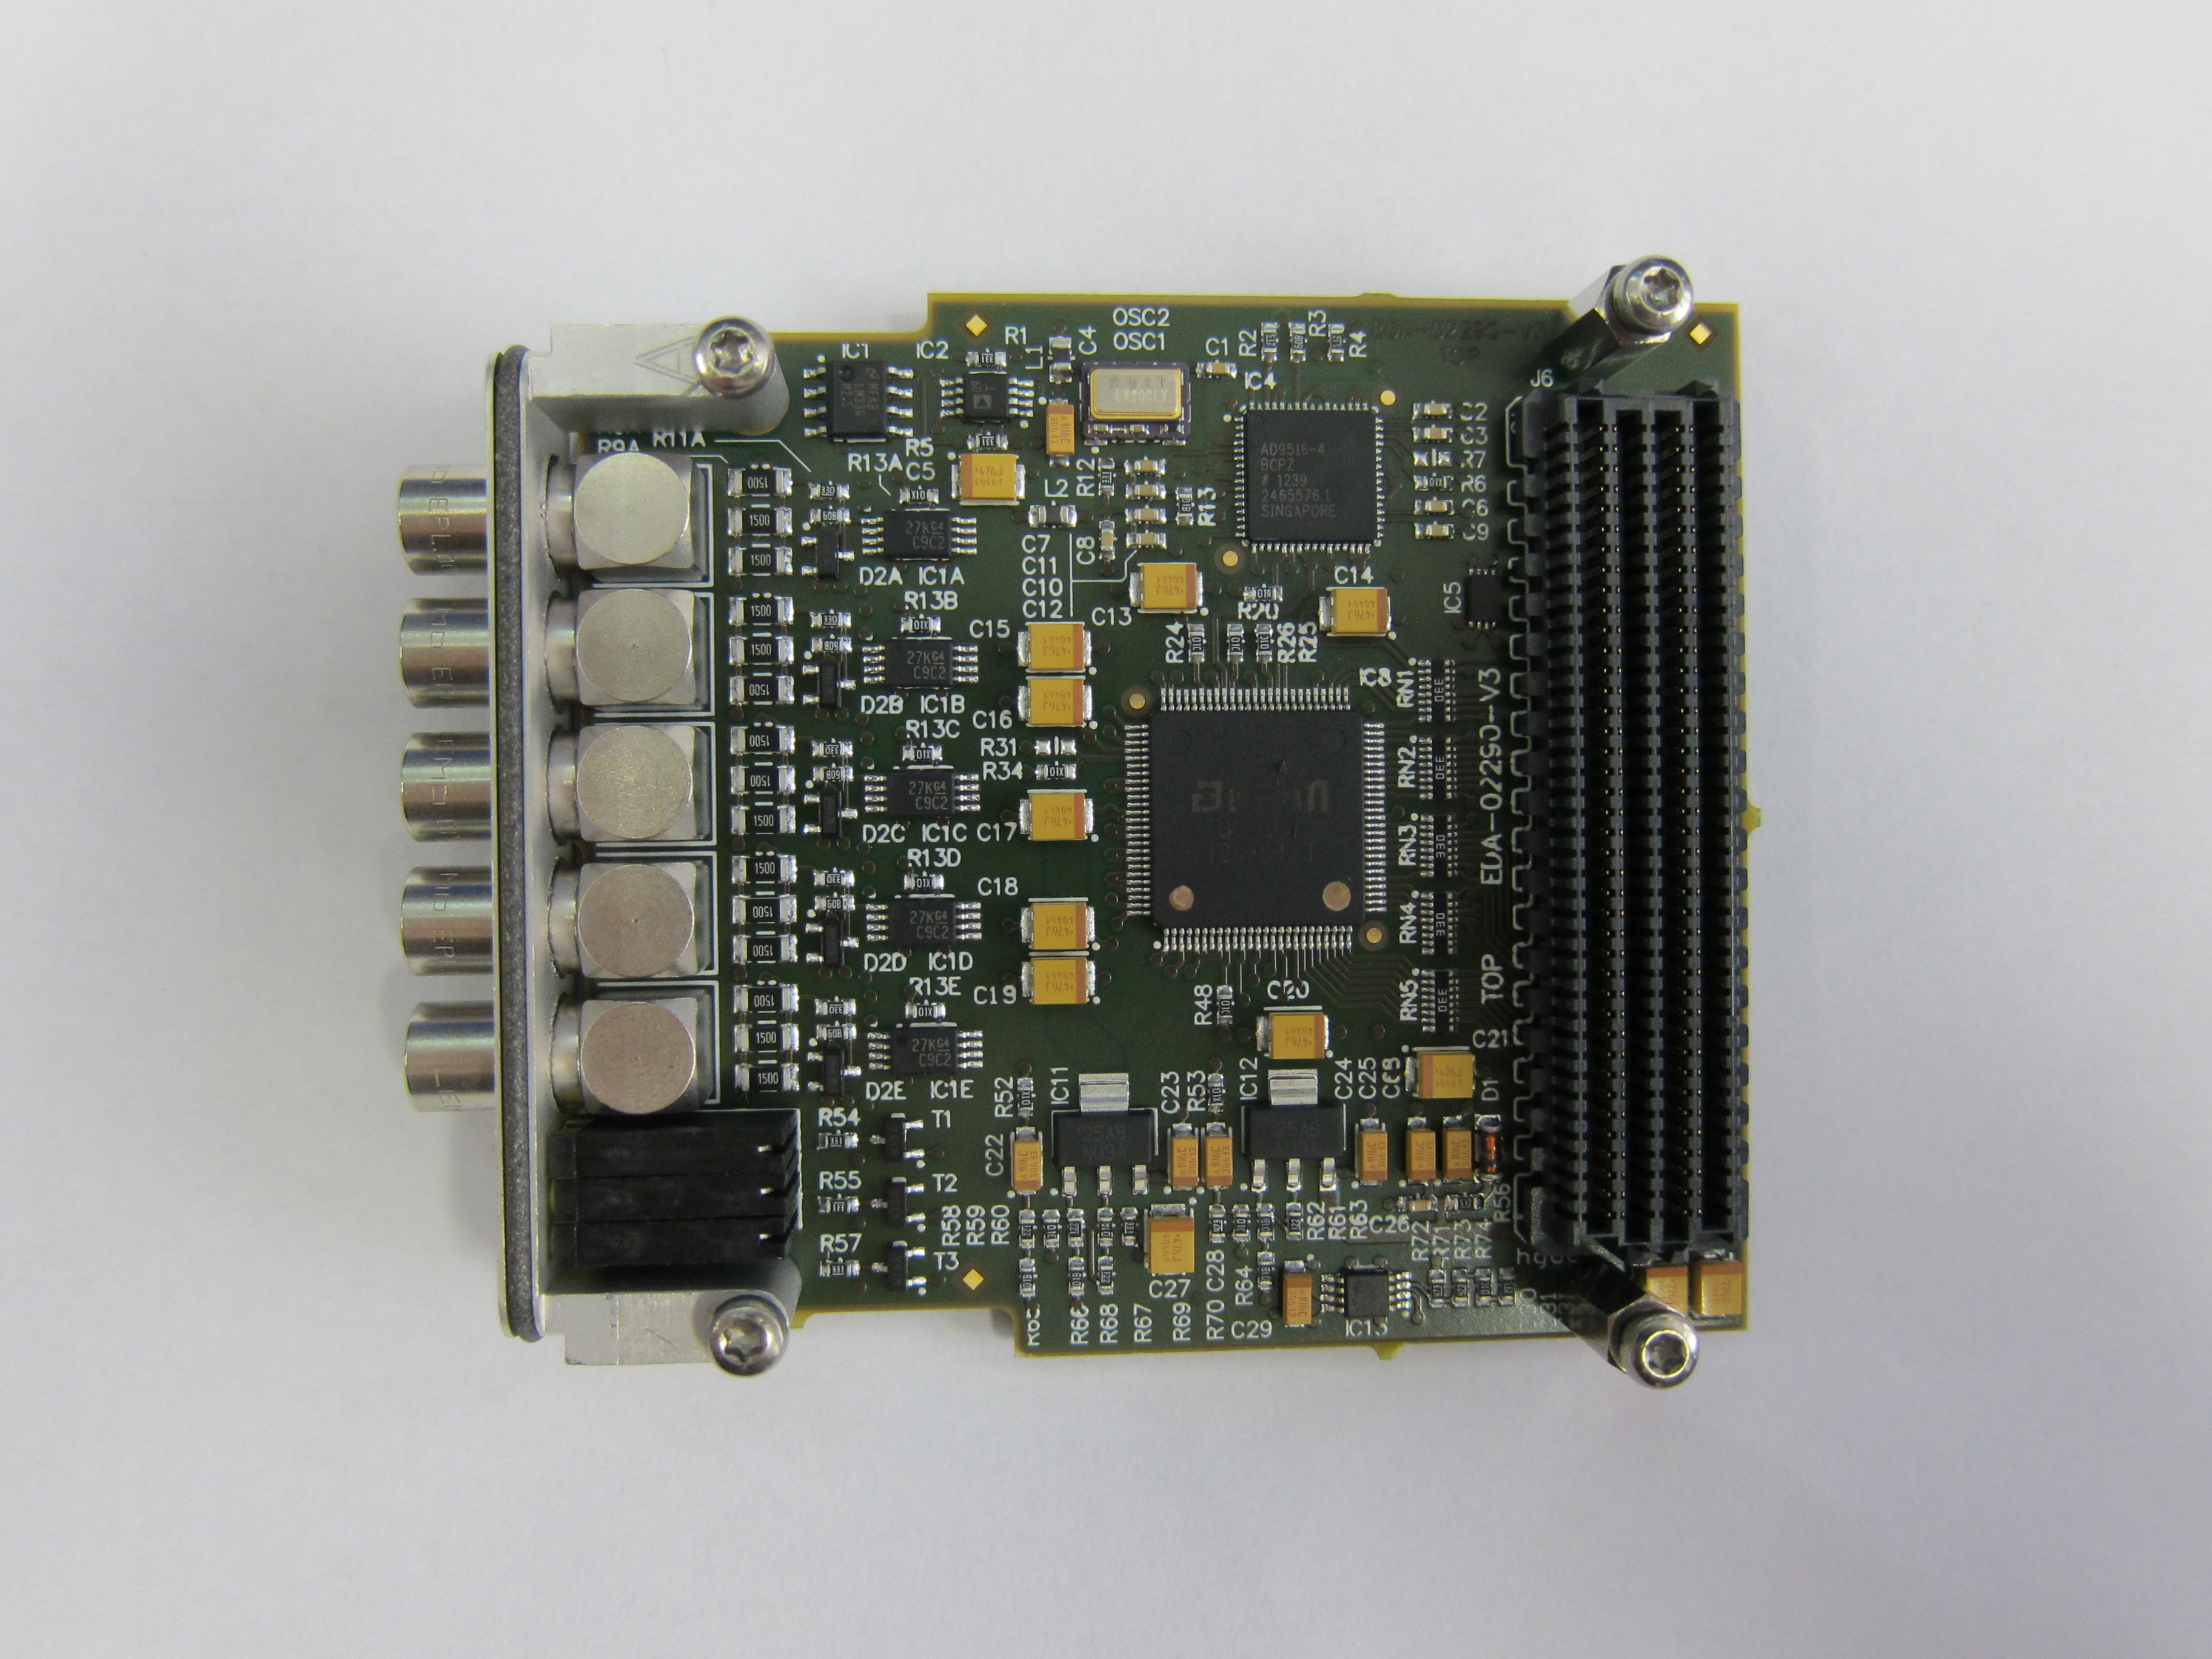
\includegraphics[height=4cm]{../pictures/fmc-tdc.eps}
  \end{center}

  \note[item]{This is the TDC mezzanine, developed in collaboration with other groups at CERN.}

\end{frame}

%------------ FRAME --------------------------------------------------
\begin{frame}{FMC mezzanine: 100 MSPS 14-bit 4-channel ADC}

  \begin{center}
    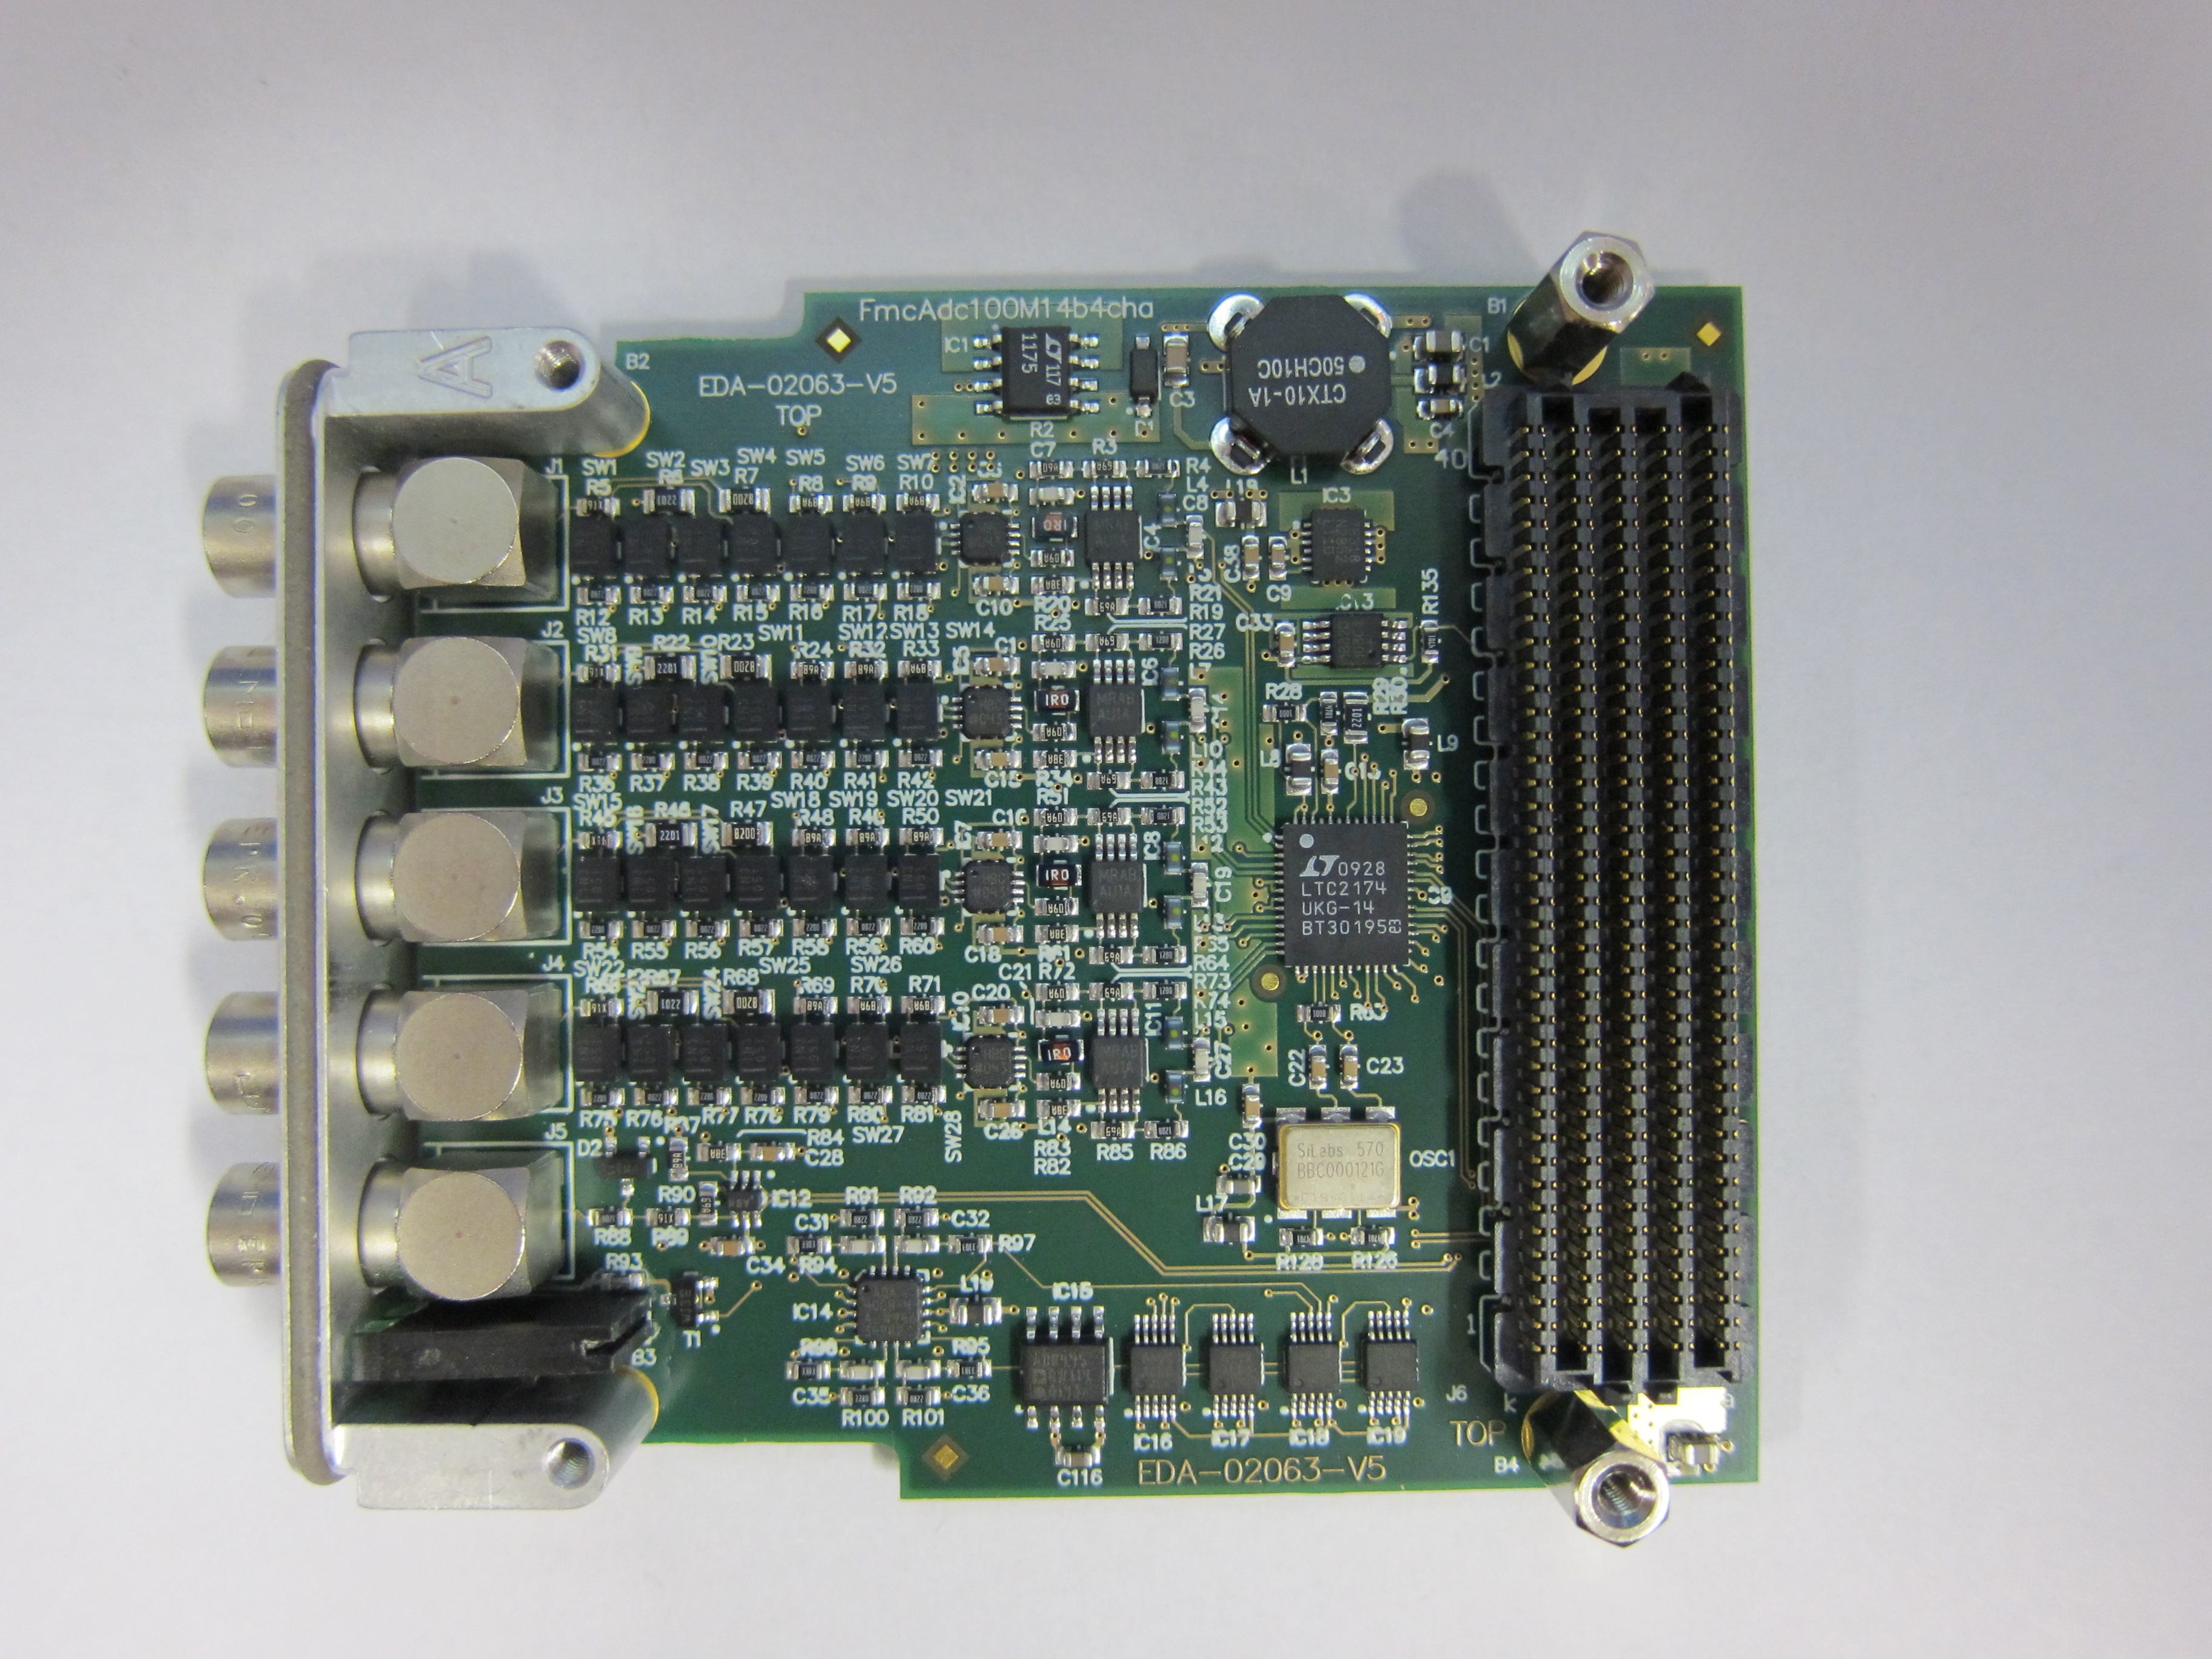
\includegraphics[height=4cm]{../pictures/fmc-adc-100m.eps}
  \end{center}

  \note[item]{And this is our ADC mezzanine, with oscilloscope-like analogue front-end}

\end{frame}

%------------ FRAME --------------------------------------------------
\begin{frame}{Commercially available CERN OH designs}{September 2013}

  \begin{table}
    \centering
    \begin{tabular}{|l||r|r|r|}
      \hline
      Project & Producers & Users & Produced\\
      \hline\hline
      SPEC carrier - PCIe & 3 & 41 & 300 \\
      \hline
      SVEC carrier - VME & 2 & 4 & 105 \\
      \hline
      SPEXI carrier - PXIe & 1 & 2 & (proto) 3 \\
      \hline
      \hline
      ADC 100M 14b 4ch & 2 & 11 & 70 \\
      \hline
      TDC 1ns 5cha & 1 & 3 & 70 \\
      \hline
      FMC DEL 1ns 4cha & 3 & 4 & 108 \\
      \hline
      FMC DIO 5ch & 3 & 10 & 92 \\
      \hline
      \hline
      \textit{WR switch 18 ports} & 1 & 11 & 77\\
      \hline
    \end{tabular}
    \caption{eight CERN OH designs found producers and users}
  \end{table}

  \note[item]{Here is a summary of CERN designs commercially available.}
  \note[item]{As you can see, most of the boards have more than one producer.}
  \note[item]{And for the more generic boards, the number of user is quite big.}

\end{frame}


%#####################################################################
%############ SECTION ################################################
\section{Gateware architecture}

\subsection*{} % dummy subsection to display dots

%------------ FRAME --------------------------------------------------
\begin{frame}{Gateware architecture}

  \begin{block}{Wishbone for modularity}
    \begin{itemize}
    \item Open standard
    \item Simple, uses few FPGA resources
    \item Collection of cores already available (OpenCores)
    \end{itemize}
  \end{block}

  \begin{block}{New cores developed}
    \begin{itemize}
    \item At CERN: VME64x, PCIe, DDR3
    \item By collaborators: Wishbone crossbar (GSI)
%    \item Crossbar to interconnect/arbitrate masters and slaves % developed in GSI
    \end{itemize}
  \end{block}

  \note[item]{I will talk now about the gateware architecture.}
  \note[item]{We choose the Wishbone bus to interconnect the different blocks in the FPGA.}
  \note[item]{Because it's an open standard.}
  \note[item]{It's simple.}
  \note[item]{And a large collection of core already exists.}

\end{frame}

%------------ FRAME --------------------------------------------------
\begin{frame}{Example: FMC-ADC gateware architecture}

  \begin{center}
    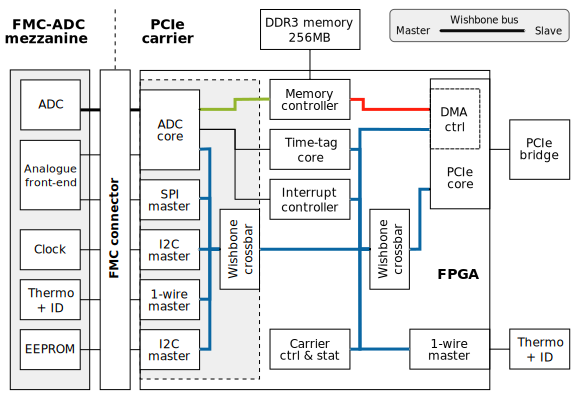
\includegraphics[height=6cm]{../pictures/spec-fmc-adc_arch_simple_color.eps}
  \end{center}

  \note[item]{Here is an example of the Wishbone architecture.}
  \note[item]{It represents the FMC-ADC gateware for a PCIe carrier.}
  \note[item]{Several Wishbone buses interconnects every cores, it makes the design very modular.}

\end{frame}


%#####################################################################
%############ SECTION ################################################
\section{New tools}

\subsection*{} % dummy subsection to display dots

%------------ FRAME --------------------------------------------------
\begin{frame}{Gateware design tools}

  \begin{block}{hdlmake: Automates design flow}
    \begin{itemize}
    \item Generates Makefiles for synthesis and simulation.
    \item Project structure described in Manifest files.
    \item Solves dependencies (fetches remote ones).
    \end{itemize}
  \end{block}

  \begin{block}{wbgen2: Wishbone slave generator}
    \begin{itemize}
    \item Generates registers, RAM, FIFO, interrupt controller.
    \item Describes structure in a single text file.
    \item Automatically generates HDL source, C header and documentation.
    \end{itemize}
  \end{block}

  \note[item]{To help with the gateware design, we also developed some tools.}
  \note[item]{The first one is hdlmake. It allows to generate Makefile for synthesis and simulation from a Manifest file describing the project structure.}
  \note[item]{The second one is wbgen2, which is a Wishbone slave generator.}
  \note[item]{It generate the HDL and C header source and documentation from a single text file.}
  \note[item]{They are both available on the OHWR website.}

\end{frame}

%------------ FRAME --------------------------------------------------
\begin{frame}{wbgen2: HTML documentation example}

  \begin{center}
    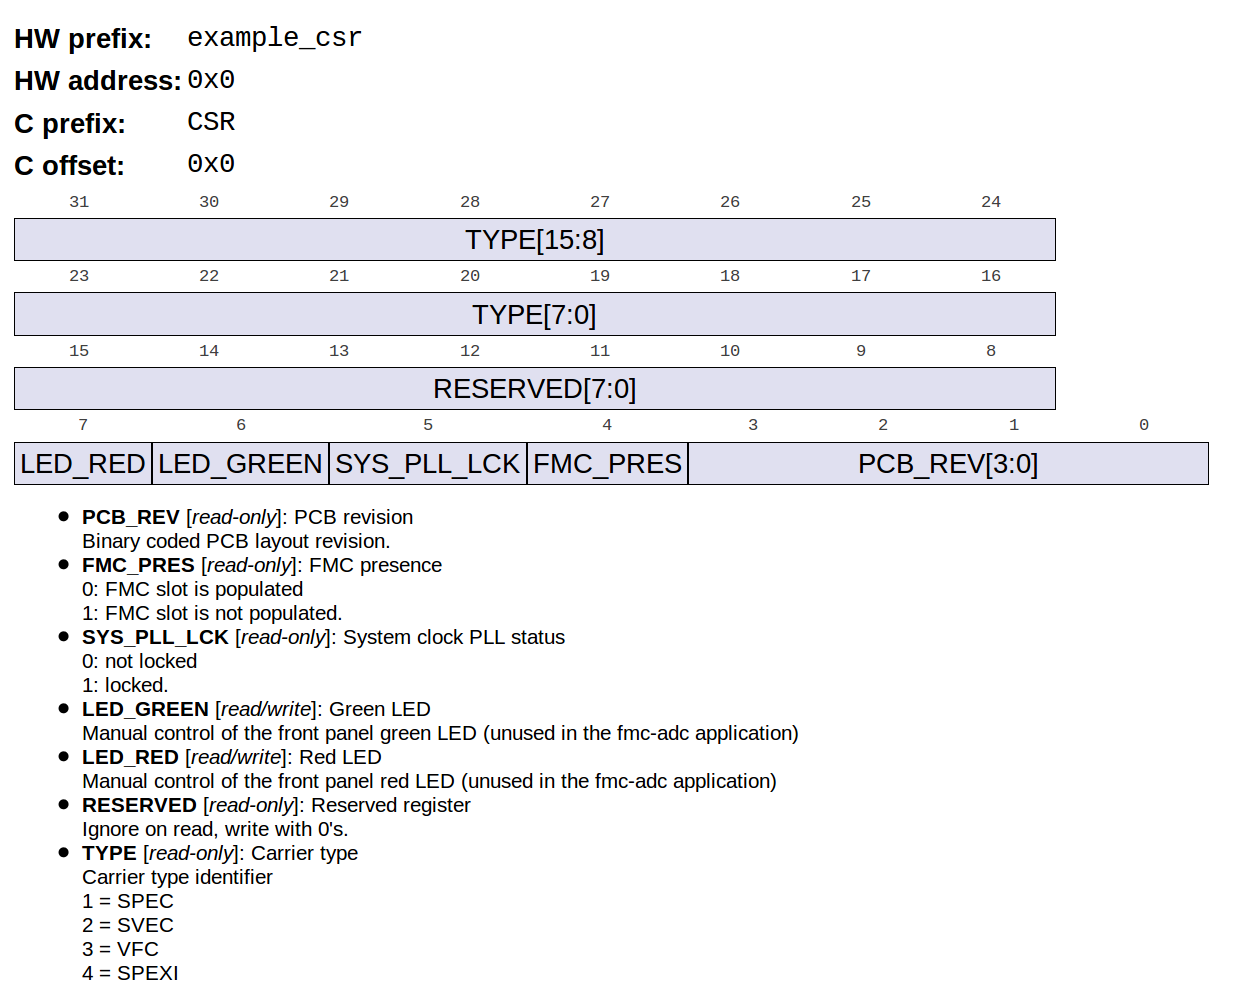
\includegraphics[height=7cm]{../pictures/wbgen_example.eps}
  \end{center}

  \note[item]{This is a example of HTML documentation AUTOMATICALLY generated by wbgen2.}

\end{frame}

%------------ FRAME --------------------------------------------------
\begin{frame}{Testing environment}

  \begin{block}{Production test systems}
    \begin{itemize}
    \item Performs automated production tests.
    \item Includes a software framework to run the tests (Python).
%    \item Stores calibration data in FMC EEPROM.
%    \item Generates log files (life-cycle management).
    \end{itemize}
  \end{block}

   \begin{center}
    \includegraphics[height=5cm]{../pictures/pts_rack.eps}
  \end{center}

% Before CERN was testing boards
% -> unloads CERN team

% Warranty, repair of faulty boards

  \note[item]{For all the boards of our kit, we also developed a PRODUCTION test system.}
  \note[item]{We developed a software framework in Python to run the tests.}
  \note[item]{(After passing on the test system, the boards are ready to be put in stock.)}

\end{frame}

\begin{comment}
%------------ FRAME --------------------------------------------------
\begin{frame}{Example: VME boards test system}

  \begin{center}
    \includegraphics[height=6.5cm]{../pictures/pts_rack.eps}
  \end{center}

  \note[item]{This is an example of a test system. This one is for VME boards.}
  \note[item]{This is where we insert the board to test.}
  \note[item]{We can see here a bar-code reader, to scan the serial number of each board.}
  \note[item]{And this is a laptop that manages system.}

\end{frame}
\end{comment}

\begin{comment}
%------------ FRAME --------------------------------------------------
\begin{frame}{New concepts}

  \begin{block}{SDB: Self Describing Bus}
    \begin{itemize}
    \item Allows software to know about gateware architecture
    \item Series of predefined structures
    \item Contains meta-data about HDL cores
    \end{itemize}
  \end{block}

  \begin{block}{SDB File System}
    \begin{itemize}
    \item Based on SDB data structures
    \item Easy to parse (e.g. for embedded processor)
    \item Library and tools available % (generate, read)
    \item Used in the FMC EEPROM
    \end{itemize}
  \end{block}

  \note[item]{During the kit design we implemented some new concepts.}
  \note[item]{This first one is SDB, for Self Describing Bus.}
  \note[item]{It allow the driver to know about the gateware just by accessing a set of structure in the HDL cores.}
  \note[item]{The second concept is a file system derived from SDB.}
  \note[item]{It's a very simple filesystem than can be read by an embedded processor and it's used for example in the FMC EEPROM.}

\end{frame}
\end{comment}


%#####################################################################
%############ SECTION ################################################
\section{Future work \& conclusions}

\subsection*{} % dummy subsection to display dots

%------------ FRAME --------------------------------------------------
\begin{frame}{Future work}

  \begin{block}{Consolidate our designs}
    \begin{itemize}
    \item Consolidate gateware and drivers. Make more releases.
    \item Consolidate documentation (manuals, FAQs, ...).
    \item Help companies to provide support.
    \end{itemize}
  \end{block}

  \begin{block}{Facilitate sharing with FOSS EDA tools}
    % FOSS = Free Open Source Software, EDA = Electronic Design Automation
    \begin{itemize}
    \item Tools are expensive and do not interoperate.
    \item Existing FOSS tools not usable for complex designs.
    \item We contribute to the development of FOSS tools:
      \begin{itemize}
      \item Extension of \textbf{Icarus} Verilog simulator with VHDL and \\ SystemVerilog support.
      \item Enhancement of \textbf{KiCAD} (schematics \& PCB editor).
      \end{itemize}
    \end{itemize}
  \end{block}

  \note[item]{For the last 4 years the focus was on make the kit commercially available, but now we still have to consolidate the design.}
  \note[item]{And also help companies selling our board to provide support to other users.}
  \note[item]{Finally, we also contribute to Free Open Source Software EDA tools.}
  \note[item]{Because the EDA tools license are expensive and the different tools don't interoperate.}
  \note[item]{And the FOSS are not usable for complex designs.}
  \note[item]{So we contribute to the Icarus simulator to add support for VHDL and SystemVerilog.}
  \note[item]{And also to KiCAD a PCB design tool.}

\end{frame}

%------------ FRAME --------------------------------------------------
\begin{frame}{Conclusions}

  \begin{block}{}
    \begin{itemize}
    \item CERN's FMC kit is not only a set of hardware modules.
      \begin{itemize}
      \item HDL cores, drivers, test system, tools
      \item Commercially available (sometimes from several sources)
      \end{itemize}
    \item Open Hardware has many advantages.
      \begin{itemize}
      \item Anyone can help in developments and make improvements.
%      \item Allows to work differently with industry. % (design work, smaller companies).
      \item Not tied to a single company for production and support.
      \end{itemize}
%    \item Using standards attracts users and improves re-usability. %(VME64x, PCIe, FMC, Wishbone)
    \item OHR site is practical for engineers and is stimulating.
%    \item Eight CERN designs are already commercialized.
    \item New users and collaborations are welcome.
%    \item OHR site contains many re-usable HDL cores.
%    \item Good FOSS tools needed to facilitate sharing.
%    \item Many designs being developed and several are already produced by industry.
    \item Four years of experience show it works!
    \end{itemize}
  \end{block}

  \begin{block}{}
    \begin{center}
    Want to know more? Take a tour on \textbf{ohwr.org}
    \end{center}
  \end{block}

  \note[item]{}

\end{frame}


%------------ FRAME --------------------------------------------------
%?? Erik's slide with products webpages?



%\vspace{0.2cm}
%Opening up your designs does make you more vulnerable to this disease.
%\end{frame}
%%One slide to justify our license choice so far
%% One slide on evil patents and the risk for open design.

\end{document}


